\documentclass[]{article}

\usepackage{graphicx}
\usepackage{placeins}
\usepackage{amsmath,amssymb}
\usepackage[colorlinks=true,citecolor=red]{hyperref}
\usepackage{siunitx}
\usepackage{listings}

\usepackage{geometry}
\geometry{a4paper,margin=1in,portrait}

\usepackage{tikz}
\usetikzlibrary{arrows,decorations.pathmorphing,backgrounds,positioning,fit}
\tikzset{module/.style={minimum size = 15mm,rectangle,draw=black,thick,fill=blue!20},
		pre/.style={<-,shorten <=1pt,>=stealth',semithick},
		post/.style={->,shorten <=1pt,>=stealth',semithick}}

\allowdisplaybreaks

\begin{document}
\title{Documentation for digital pattern generator-based imaging controller}
\author{Ryan Thomas}
\date{\today}
\maketitle

\section{Introduction}
\label{sec:introduction}
This document describes the design and operation of the digital pattern generator (DPG)-based imaging controller used in the Kj{\ae}rgaard lab.  While both this controller and its predecessor are implemented using a field-programmable gate array (FPGA), namely the Xlinx Spartan 3AN development board, the DPG imaging controller has a much simpler FPGA architecture and is more easily customizable than the previous, bespoke version.

Whereas the previous imaging controller had many different modules, each of which controlled a different aspect of the timing sequence, the DPG solution has only two modules: the DPG itself and a module to generate triggers for the FlexDDS.  The reason that these are separate is that we need millions of triggers for the FlexDDS at a fixed rate and duty cycle, and using a DPG to generate these would require an enormous amount of memory.  It is easier to use a dedicated module for this purpose.
\begin{figure}[htbp]
	\centering
	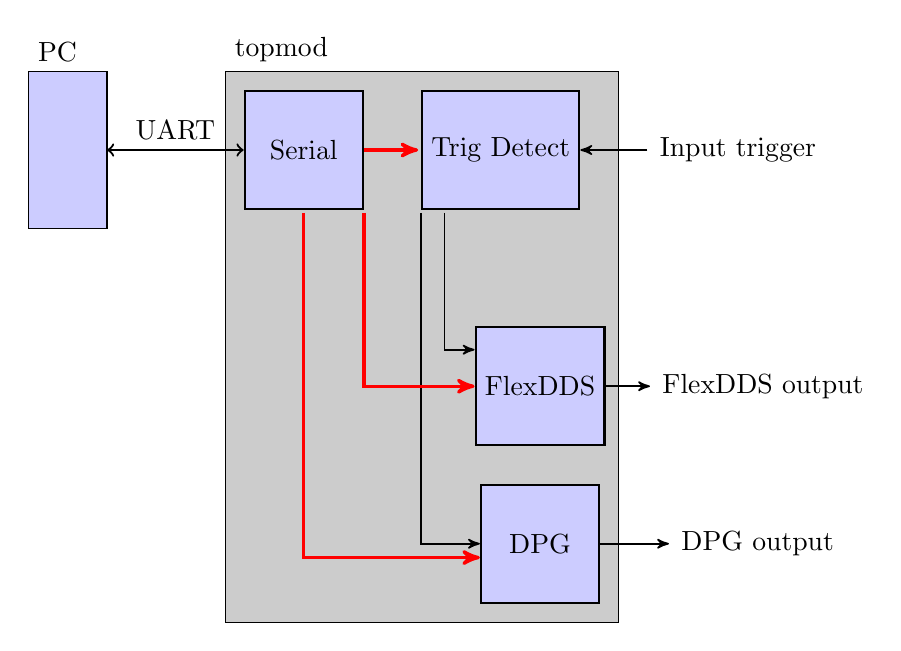
\begin{tikzpicture}
		\draw[fill=black!20] (0,0) rectangle (5,7);
		\node[anchor=south west] (topmod) at (0,7) {topmod};
		\draw[fill=blue!20] (-2.5,5) rectangle (-1.5,7);
		\node[anchor=south west] (pc) at (-2.5,7) {PC};
		\node[module] (serial) at (1,6) {Serial};
		\draw[<->,thick] (-1.5,6) -- node[above] {UART} (serial.west);
%		node[module] (serial) at ++(1,0) {Serial};
%		\node[module] (serial) at (1,6) {Serial} edge[pre] node[anchor=south] {UART} (pc);
		\node[module] (trig-detect) at (3.5,6) {Trig Detect} edge[pre,red,very thick] (serial);
		\node[module] (flexdds) at (4,3) {FlexDDS};
		\node[module] (dpg) at (4,1) {DPG};
		\draw[post] ([xshift=3mm]trig-detect.south west) |- ([yshift=-3mm]flexdds.north west);
		\draw[post] (trig-detect.south west) |- (dpg.west);
		\draw[post,red,very thick] (serial.south east) |- (flexdds.west);
		\draw[post,red,very thick] (serial.south) |- ([yshift=-5]dpg.west);
		
		\node[] (trigin) at ([xshift=2cm]trig-detect.east) {Input trigger} edge[post] (trig-detect.east);
		\node[] (flexdds-out) at ([xshift=2cm]flexdds.east) {FlexDDS output} edge[pre] (flexdds.east);
		\node[] (dpg-out) at ([xshift=2cm]dpg.east) {DPG output} edge[pre] (dpg.east);

	\end{tikzpicture}
	\caption{Diagram of the DPG-based imaging controller. A PC transmits parameters to the FlexDDS trigger generator and a digital pattern to the DPG.  The sequence starts either when an input trigger is received or when a software trigger is issued by the host PC over serial.  Thick red lines indicate the transmission of information to and from the serial controller.}
	\label{fg:diagram}
\end{figure}

\section{Hardware}
\label{sec:hardware}
\subsection{Digital Pattern Generator (DPG)}
\label{ssec:dpg}
A DPG is simple to understand -- it is a device that stores a list of digital output patterns and the times at which they should be enacted.  In the case of the current DPG, these are stored as a series of 40-bit (5 byte) instructions, where the most-significant byte (MSB) is the type of instruction and bytes 0 to 3 (for a total of 32 bits) are the \emph{data}.  There are currently three types of instructions:
\begin{enumerate}
	\item $\mathrm{MSB} = 0\mathrm{x}00$ This instruction tells the DPG to wait for a time equal to \emph{data} sample clock cycles.
	\item $\mathrm{MSB} = 0\mathrm{x}01$ This instruction tells the DPG to output the pattern equal to \emph{data}.
	\item $\mathrm{MSB} = 0\mathrm{x}02$ This instruction tells the DPG to wait for a digital input event before continuing to the next instruction.  Bits 0 to 3 of \emph{data}, interpreted as an unsigned integer, indicate the digital input channel to look at, and bits 8 to 9 indicate the type of edge to look for.
\end{enumerate}
\begin{figure}
	\centering
	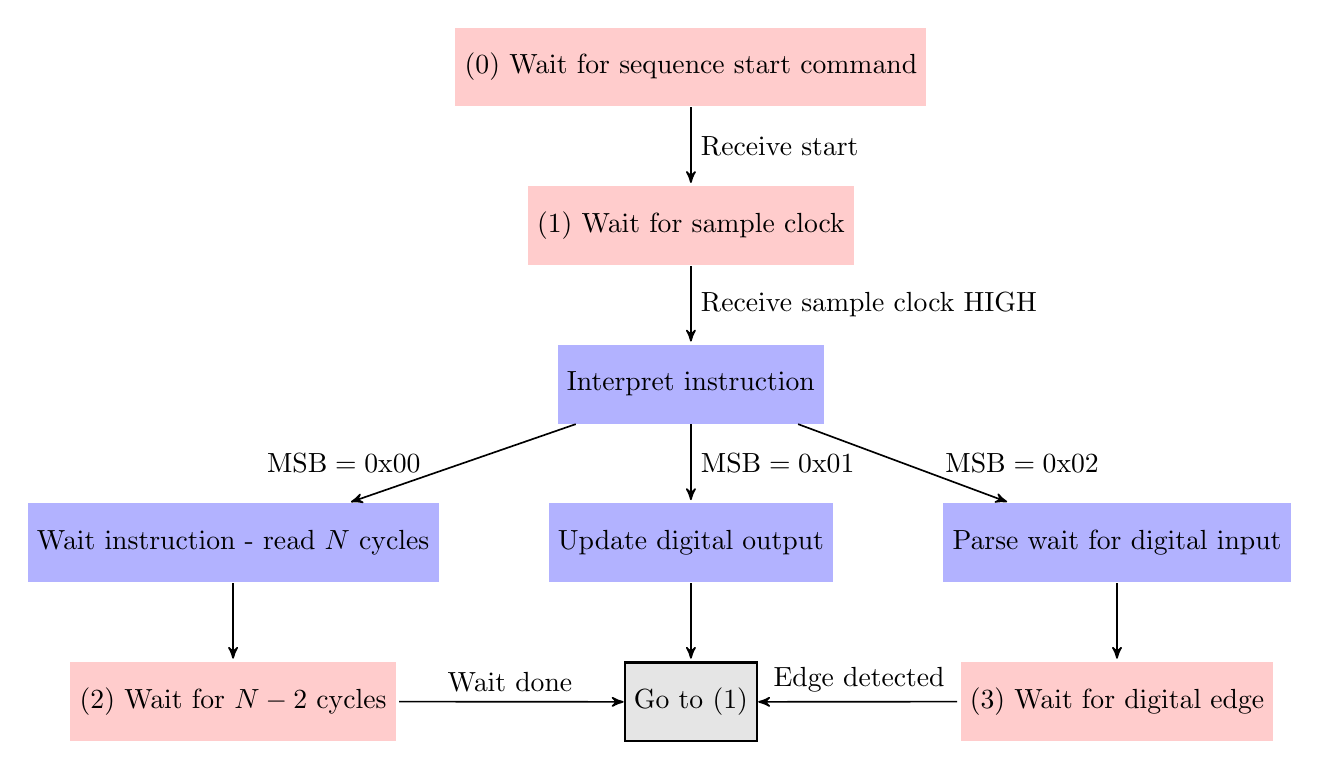
\begin{tikzpicture}[node distance=10mm and 15mm,
		state/.style={rectangle,fill=red!20,minimum size=10mm},
		cond/.style={rectangle,fill=blue!30,minimum size=10mm},
		goto/.style={rectangle,fill=black!10,draw=black,thick,minimum size=10mm}]
		\node[state] (wait-for-start) at (0,0) {(0) Wait for sequence start command};
		\node[state] (wait-for-sample-clock) [below=of wait-for-start] {(1) Wait for sample clock} edge[pre] node[anchor=west] {Receive start} (wait-for-start);
		\node[cond] (interpret-instruction) [below=of wait-for-sample-clock] {Interpret instruction} edge[pre] node[anchor=west] {Receive sample clock HIGH} (wait-for-sample-clock);
		
		\node[cond] (wait) [below left=of interpret-instruction] {Wait instruction - read $N$ cycles} edge[pre] node[left=4mm,anchor=east] {$\mathrm{MSB}=0\mathrm{x}00$} (interpret-instruction);
		\node[state] (wait-for) [below=of wait] {(2) Wait for $N-2$ cycles} edge[pre] node[anchor=east] {} (wait);
		
		\node[cond] (digital-out) [below=of interpret-instruction] {Update digital output}
		edge[pre] node[anchor=west] {$\mathrm{MSB}=0\mathrm{x}01$} (interpret-instruction);
		\node[goto] (goto-1) [below=of digital-out] {Go to (1)} edge[pre] (digital-out);
		\draw[post] (wait-for) -- node[above] {Wait done} (goto-1);
		
		\node[cond,node distance=10mm and 15mm] (wait-input) [below right=of interpret-instruction] {Parse wait for digital input} edge[pre] node[right=4mm,anchor=west] {$\mathrm{MSB}=0\mathrm{x}02$} (interpret-instruction);
		\node[state] (wait-edge) [below=of wait-input] {(3) Wait for digital edge} edge[pre] (wait-input);
		\draw[post] (wait-edge) -- node[above] {Edge detected} (goto-1);
		
%		\node[cond,node distance=10mm and 20mm] (seq-stop) [right=of wait-for-sample-clock] {Sequence stopped} edge[pre] node[anchor=south] {Empty instructions} (wait-for-sample-clock);
%		\draw[post] (seq-stop.north) |- (wait-for-start.east);
	\end{tikzpicture}
	\caption{Diagram of the finite-state machine (FSM) at the heart of the DPG.  Red boxes indicate states of the state machine; blue boxes indicate conditional statements.  New instructions are requested when a ``start'' command is received and also whenever a sample clock HIGH is detected.  When all instructions are read, the FSM returns to state 1.  If a sequence ``stop'' command is received, the controller returns to state 0.}
	\label{fg:dpg}
\end{figure}

At the heart of the DPG is a finite-state machine (FSM) that executes the reads, parses, and executes new instructions: a diagram is shown in Fig.~\ref{fg:dpg}.  The idle state of the DPG is the ``wait-for-start'' state, where the FSM waits for the sequence start command from the PC over the UART (serial) connection.  When it receives this trigger, it raises the \verb|seqEnabled| signal and request a new instruction from the block memory that holds the instruction list.  Raising \verb|seqEnabled| enables the detection of input triggers, and when the input trigger is received the sample clock starts.  The sample clock is set to $1/4$ of the FPGA master clock (but with a duty cycle of $1/4$), so with the current master clock frequency of 100 MHz the sample clock is 25 MHz.  This means that new instructions are processed every 40 ns.  The factor of $1/4$ was chosen to ensure that there is sufficient time to read new instructions from the memory between successive sample clock edges.

When the FSM detects that the sample clock is high it issues a request for a new instruction at the same time that it parses the current one.  When the current instruction number, given by the memory address, is less than the number of stored instructions the FSM also raises the \verb|seqRunning| signal which tells the sample clock generator to continue running.  If the current instruction number is equal to the maximum address, the FSM raises the \verb|seqDone| signal which tells the controller on the next sample clock edge to read the first instruction again and return to the ``wait-for-sample-clock'' state (state 1 in Fig.~\ref{fg:dpg}).  If at any time a ``sequence stop'' command is received, the FSM immediately returns to the idle state (state 0).

If the current instruction is a digital output instruction, the controller routes the \emph{data} part of the instruction to the signal \verb|dOutSig|, which is routed to the physical output when \verb|seqRunning| is high.  If \verb|seqRunning| is low, then the digital output is routed from the signal \verb|dOutManual| which is the manually set value.  This signal can either be a default output state, or the user can set it as needed for testing.  

If the current instruction is a wait instruction, the FSM reads the wait time from \emph{data} as a delay of $N$ sample clock cycles, where $N$ is a 32-bit unsigned integer.  The FSM proceeds to the ``wait'' state (state 2) and waits for $N-2$ cycles - the $-2$ is necessary to account for the sample period during which the instruction is parsed and the periods during which the counting is done.  By choosing to wait for $N-2$, the delays between updates of the digital output are $N$ sample clock cycles.  Note that the controller cannot wait for 0 cycles, and asking it to wait for 1 cycle will result in it waiting for 2 cycles.  In order to have a delay of 1 cycle between successive updates to the digital output, the user should have two successive digital output instructions rather than separating them by a wait time.

Finally, if the current instruction is a wait for input instruction, the FSM reads the input bit from bits 0 to 3 of \emph{data} corresponding to an unsigned integer from 0 to 7.  The edge type to look for is encoded in bits 8 to 9 with a ``00'' being a falling edge, ``01'' being either a falling or rising edge, and ``10'' being a rising edge.  When the correct edge is detected, the FSM moves to state 1.  An edge type of ``11'' is not used and will immediately move to state 1.  Digital inputs are detected synchronously with the master clock, so any input signal must be high for at least one master clock period (10 ns).  Currently, no digital inputs are used, but this should be relatively easy to change in the future if needed.

\subsubsection{Programming the DPG}
\label{sssec:programming-dpg}
The DPG is programmed using a relatively simple set of commands which are sent to the FPGA using a serial (UART) connection.  Commands are interpreted least-significant bit (and byte) first.  Some commands set the controller up to read the next command(s) as a numerical parameter, or, in the case of memory uploading, the next series of commands as writes to memory.  A table of commands is given in Table~\ref{tb:commands}
\begin{table}[htbp]
	\centering
	\begin{tabular}{c|c|p{5cm}}
		Command							&	Action													&	Subsequent command(s)\\\hline
		$0\mathrm{xID}\_00\_00\_00$		&	Sequence start											&	None\\\hline
		$0\mathrm{xID}\_00\_00\_01$		&	Sequence stop											&	None\\\hline
		$0\mathrm{xID}\_00\_00\_02$		&	Sends status information back to PC						&	None\\\hline
		$0\mathrm{xID}\_00\_00\_03$		&	Sends current value of \verb|dOutManual| back to PC		&	None\\\hline
		$0\mathrm{xID}\_01\_00\_00$		&	Set value of \verb|dOutManual|							&	Next 32-bit command is interpreted as \verb|dOutManual|\\\hline
		$0\mathrm{xID}\_02\_xx\_xx$		&	Upload instructions to memory - see text				&	Next $0\mathrm{x}00\_00\_xx\_xx$ commands must be 40-bits - see text\\\hline
	\end{tabular}
	\caption{Command options for DPG.  ID is the DPG's serial ID, currently set to $00$.}
	\label{tb:commands}
\end{table}
Status information from the DPG is sent with the two most-significant bits being the value of \verb|seqEnabled| and \verb|seqRunning|, respectively, and the remaining bits represent the address in memory that is currently being accessed.

Uploading instructions to memory is slightly different from other commands.  To upload instructions to memory, one first needs to send the command $0\mathrm{xID}\_02\_xx\_xx$ to the FPGA where $xx\_xx$ is the hexadecimal representation of the number of instructions $N_{\rm instr}-1$ that will be sent to the FPGA, where $N_{\rm instr}$ is the number of instructions.  Currently, the block memory where these instructions reside can handle up to $2^11=2048$ instructions, but one can change that in VHDL if more instructions are necessary.  Obviously with the current encoding scheme the maximum number of instructions that can be stored is $2^{16}=65536$, although other encoding schemes could be used.  Once the previous command is sent and the FPGA is primed to receive instructions to write to memory, the user must transmit $N_{\rm instr}$ 40-bit instructions in least-significant bit first format (little endian), where the least 32 significant bits are the data and the most-significant byte is the instruction type.  A typical set of instructions for programming the DPG could be
\begin{align}
\textrm{Stop DPG}\quad\quad&0\mathrm{x}00\_00\_00\_01\notag\\
\textrm{Prime for receiving manual values}\quad\quad&0\mathrm{x}00\_01\_00\_00\notag\\
\textrm{Send default values (all 0)}\quad\quad&0\mathrm{x}00\_00\_00\_00\notag\\
\textrm{Prime for receiving 10 instructions}\quad\quad&0\mathrm{x}00\_02\_00\_09\notag\\
\textrm{Set all outputs to 0}\quad\quad&0\mathrm{x}01\_00\_00\_00\_00\notag\\
\textrm{Wait 10 cycles}\quad\quad&0\mathrm{x}00\_00\_00\_00\_0\mathrm{A}\notag\\
\textrm{Raise bit 0}\quad\quad&0\mathrm{x}01\_00\_00\_00\_01\notag\\
\textrm{Wait 2 cycles}\quad\quad&0\mathrm{x}00\_00\_00\_00\_02\notag\\
\textrm{Raise bits 31 and 15}\quad\quad&0\mathrm{x}01\_80\_00\_80\_01\notag\\
\textrm{Wait 20 cycles}\quad\quad&0\mathrm{x}00\_00\_00\_00\_14\notag\\
\textrm{Lower bit 31, raise bit 1}\quad\quad&0\mathrm{x}01\_00\_00\_80\_03\notag\\
\textrm{Wait 1 cycle, lower bit 1}\quad\quad&0\mathrm{x}01\_00\_00\_80\_01\notag\\
\textrm{Wait for rising edge on input 0}\quad\quad&0\mathrm{x}02\_00\_00\_00\_20\notag\\
\textrm{Lower all bits}\quad\quad&0\mathrm{x}01\_00\_00\_00\_00\notag\\
\textrm{Start DPG}\quad\quad&0\mathrm{x}00\_00\_00\_00\notag
\end{align}
It is not strictly required that one stop the DPG before uploading instructions, but if one does not then there could potentially be read/write conflicts if the DPG receives a trigger while instructions are being uploaded.  Additionally, if the first instruction changes between uploads and the DPG is \emph{not} stopped beforehand, then the first DPG instruction will be incorrect as it is pre-loaded on receipt of a ``start'' command.

\subsection{FlexDDS trigger system}
\label{ssec:flexdds}
The imaging controller is also used to generate triggers for the FlexDDS.  Since we generate several seconds worth of triggers at 200 kHz for three channels, it makes sense to not have these be part of the DPG.  Instead, it is a separate module in the FPGA architecture.  The FlexDDS system has a serial ID of $0\mathrm{x}01$, and serial commands can be found in Table~\ref{tb:flexdds}.
\begin{table}[htbp]
	\centering
	\begin{tabular}{c|c|p{5cm}}
		Command							&	Action													&	Subsequent command(s)\\\hline
		$0\mathrm{xID}\_00\_xx\_00$		&	Pulse period for output $0\mathrm{x}xx$.				&	Next 32-bit command is pulse period in FPGA master clock cycles\\\hline
		$0\mathrm{xID}\_00\_xx\_01$		&	Number of pulses for output $0\mathrm{x}xx$.			&	Next 32-bit command is the number of pulses\\\hline
	\end{tabular}
	\caption{Command options for FlexDDS system.  The output (0 to 2) is set with bits 8 to 15 of the initial command.}
	\label{tb:flexdds}
\end{table}
There are three FlexDDS triggers, and each can be addressed individually.  For example, to set the pulse period and number of pulses for output 1 to 5 \si{\micro\second} (200 kHz) and $2\times 10^6$ triggers the user would send
\begin{align}
\textrm{Prime for receiving pulse period}\quad\quad&0\mathrm{x}01\_00\_01\_00\notag\\
\textrm{Set pulse period to 200 kHz (100 MHz master clock)}\quad\quad&0\mathrm{x}00\_00\_01\_\mathrm{F}4\notag\\
\textrm{Prime for receiving number of pulses}\quad\quad&0\mathrm{x}01\_00\_01\_01\notag\\
\textrm{Set number of pulses to }2\times10^6\quad\quad&0\mathrm{x}00\_1\mathrm{E}\_84\_80\notag
\end{align}
The FlexDDS triggers are started whenever the input trigger signal is raised high.

\subsection{Top-level FPGA architecture}
\label{ssec:top-fpga}
There is very little in the top-level module for this FPGA architecture.  One of the main parts is a mapping of signals from the DPG to sensible names: for instance, bit 0 of the DPG output is mapped to the Andor camera trigger, and bit 1 is mapped to the Rb AOM on/off switch.  Note that many signals, such as AOM and shutter on/off signals, have inputs as well, and these are combined with the outputs from the DPG using a simple OR gate.

Another important part is the input trigger synchronization process.  This process takes the asynchronous, external input trigger and an external trigger enable signal, and creates a synchronous internal trigger signal on the rising edge of the external trigger when the enable trigger signal is high.  

Alternatively, to start the controller one can use a ``software trigger'', which is started by sending the command $0\mathrm{x}\mathrm{FF}\_00\_00\_00$ to the FPGA over serial.  This will issue an ``external'' trigger to both the FlexDDS system and the DPG simultaneously, and it can be very useful for testing.

\section{Software}
\label{sec:software}
Since programming the imaging controller uses a very simple serial interface, it should be relatively straightforward to write software in the user's preferred language that they can use to program the device.  A suite of programs has been written in MATLAB, as this is a common language in the lab.  The DPG is controlled via the two generic classes \emph{TimingController} and \emph{TimingControllerChannel}, while a more specific class for the current imaging controller is \emph{SpartanImagingController}.  The latter class is a subclass of \emph{TimingController} and mainly has named properties that are mapped to particular digital output bits.  

A slightly different class, called \emph{SpartanImaging}, provides a wrapper for an instance of \emph{SpartanImagingController} as well as an associated class for controlling the FlexDDS trigger system using the class \emph{SpartanFlexDDSTriggerSystem}.  It also has an instance of \emph{StatePrepPulses} which provides an interface for creating state-preparation pulses (microwave and radio-frequency).  

The MATLAB code has been commented so users should be able to figure out how to work the software by reading the comments and looking at examples.  Briefly, though, the \emph{TimingControllerChannel} provides the function \emph{at} that takes in a time, a value, and a time unit (default is seconds) and creates an ``event'' corresponding the change of state of that channel to \emph{value} at the specified time.  Additional functions \emph{before} and \emph{after} (with the same arguments as \emph{at}) can be used when chaining events together.  For instance, suppose one has a instance of \emph{SpartanImagingController} named \verb|sp|, and one wants to switch on the Rb probe AOM and shutter at a given time and then turn them off some time later (as would be done for imaging).  Possible code would be:
\begin{lstlisting}[language=matlab]
sp.probeRb.at(50,1,'ms').after(15,0,'us');
sp.shutterRb.anchor(50,'ms').before(2.5,1,'ms').at(sp.probeRb.last,0);
\end{lstlisting}
This code uses a number of \emph{TimingControllerChannel} functions.  In the first line, the Rb probe signal is raised high at 50 ms and then 15 \si{\micro\second} later it is lowered.  The shutter signal is slightly more complicated -- we want it to go high 2.5 ms before the probe signal (so that the shutter has sufficient time to open) and then close when the probe signal goes low.  We can use the \emph{anchor} method to set the internal channel property \verb|lastTime| to 50 ms without adding an event.  Then we can use the before function to specify an event prior to the last time added.  Note that \verb|lastTime| is the last added time, but not the last time in the sequence -- events are not sorted after each addition.  Finally, we can use the function \verb|last| to get the last time written to the probe signal and use that for specifying when the shutter signal should be lowered.  Once times are written to the channel as events they are always in seconds, so no unit is required.  The channel sequences that a user creates can be plotted using the \emph{plot} method.

The \emph{SpartanImaging} class provides familiar properties, such as cross-beam on time and time-of-flight, for the creation of standard imaging sequences.  Simply set the properties as was done in previous iterations of the controller and it should create an equivalent imaging sequence.  The \emph{SpartanImaging} class also has an \verb|expandVariables| method, just like the previous \emph{spartan} class, which means that one can specify one or more properties as vectors and the class will expand other properties to the maximum length.  

Once the properties are set, to create a basic imaging sequence one needs to run the functions
\begin{lstlisting}[language=matlab]
si.expandVariables.makeSequence.upload;
\end{lstlisting}
where \verb|si| is an instance of \emph{SpartanImaging}.  This will expand the variables, create a default sequence, and then upload that sequence to the controller or create binary files (in the case of multiple sequences).  If you want to customize the sequence, you need to do so after \verb|makeSequence| because it resets the channels and the controller.  Otherwise, you can ignore \verb|makeSequence| altogether and create a sequence from scratch.  You can take a look at the total sequence using \verb|si.plot| which will plot all channels where there are events on the same plot.  This can be crowded, so you can add an offset between each plot using \verb|si.plot(offset)| where \verb|offset| is the offset between each channel.




\end{document}

